%!TEX root = ../main.tex
\subsection{Decay time resolution}
\label{sec:b02dd:decaytimefit:resolution}

The prediction of the DTF on the decay time error is used to determine the
decay time resolution. Like in the analysis of \BdToJPsiKS (see
\cref{sec:bd2jpsiks:decaytime:resolution}) these predictions are calibrated
using linear functions with parameters $b$ and $c$. To account for different sources
introducing the decay time resolution an effective model consisting of two
Gaussians with per-event widths is used. Besides this common resolution effect
the decay time resolution model is also supposed to describe the effect of
events matched to the wrong PV which can cause a large deviation between the
true and the reconstructed decay time. The wrong PV component is
parametrised with a broad Gaussian distribution using the same mean $\mu_t$ as
the other two Gaussians and one width parameter $\sigma_{\text{PV}}$. The
complete parametrisation of the resolution model is given by
%
\begin{equation}
\begin{split}
  {\mathcal{R}}(t-t_\text{true}|\sigma_t) &= \sum_{i=1}^{2}{g_i\,\cdot\,\frac{1}{\sqrt{2\pi}(c_i + b_i \cdot \sigma_t)}\exp\left(-\frac{(t - t_\text{true} - \mu_t)^2}{2(c_i + b_i \cdot \sigma_t)^2}\right)}\\
  &+ f_{\text{PV}} \frac{1}{\sqrt{2\pi} \sigma_{\text{PV}}} \exp\left(-\frac{(t - t_\text{true} - \mu_t)^2}{2 \sigma_{\text{PV}}^2}\right) \ .
\label{eq:b02dd:decaytimefit:resolution}
\end{split}
\end{equation}
%
The first two Gaussian components have different calibration parameters $b_i$
and $c_i$ and thus different widths. Together with the fraction $f_\text{PV}$
of the wrong PV component the fractions of the two Gaussian components $g_1$
and $g_2$ sum up to unity. The shift of the Gaussian mean $\mu_t$ is shared
between all components. To extract the parameter values an unbinned maximum
likelihood fit to the simulated events where the difference between true and
reconstructed decay time is below \SI{0.4}{\ps} is performed (see
\cref{fig:b02dd:decaytimefit:resolution}). The results listed in
\cref{tab:b02dd:decaytimefit:resolution} correspond to a decay-time-resolution
related dilution of \num{0.9996}.
%
\begin{table}[!htb]
\centering
\caption{Fit parameters of decay time resolution function determined on \BdToDD signal MC.}
  \begin{tabular}{llr@{$\,\pm\,$}l}
    \toprule
    \multicolumn{2}{c}{Parameter}       &   \multicolumn{2}{c}{Value} \\
    \midrule
    $\mu_t$             &   (\si{\ps})  &   -0.00156    &   0.00023               \\
    $b_{1}$             &               &   1.022       &   0.031                 \\
    $c_{1}$             &   (\si{\ps})  &   0.0036      &   0.0012                \\
    $b_{2}$             &               &   1.24        &   0.08                  \\
    $c_{2}$             &   (\si{\ps})  &   0.0127      &   0.0035                \\
    $g_{2}$             &               &   0.23        &   0.12                  \\
    $\sigma_\text{PV}$  &   (\si{\ps})  &   0.16        &   0.04                  \\
    $f_\text{PV}$       &               &   0.0024      &   0.0014                \\
    \bottomrule
  \end{tabular}
\label{tab:b02dd:decaytimefit:resolution}
\end{table}
%
\begin{figure}[!htb]
\centering
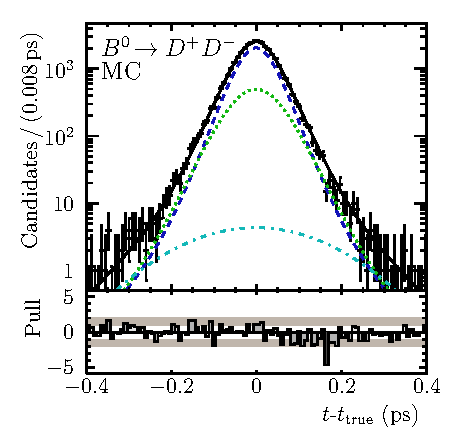
\includegraphics[width=0.5\textwidth]{07-B02DD/tikz/pdf/obsTimeErr_True_pull_logy.pdf}
\caption{Fit of per event resolution model to the difference of true and
reconstructed decay time in signal MC. The black solid line is the projection of the full
\PDF. The blue dashed and the green dotted line represent the two per-event
components and the turquoise dashed-dotted line shows the wrong PV component.}
\label{fig:b02dd:decaytimefit:resolution}
\end{figure}
%
The decay time resolution might differ between signal MC and data. In the
analysis of $\BsToDspi$ decays~\cite{LHCb-ANA-2012-068} it is found to be
$\num{1.15}$ times higher in data than in MC. If the same applied for $\BdToDD$
decays the dilution would be \num{0.9995}. This marginal difference is not expected
to influence the determination of the $\CP$ observables at all. Thus the
previously described per-event decay time resolution model without any
corrections can be used in the nominal decay time fit.
